\documentclass[a4paper,12pt]{article}
\usepackage[spanish]{babel}
\hyphenation{co-rres-pon-dien-te}
%\usepackage[latin1]{inputenc}
\usepackage[utf8]{inputenc}
\usepackage[T1]{fontenc}
\usepackage{graphicx}
\usepackage[pdftex,colorlinks=true, pdfstartview=FitH, linkcolor=blue,
citecolor=blue, urlcolor=blue, pdfpagemode=UseOutlines, pdfauthor={H. Asorey},
pdftitle={Física 1A - Guía 04}]{hyperref}
\usepackage[adobe-utopia]{mathdesign}

\hoffset -1.23cm
\textwidth 16.5cm
\voffset -2.0cm
\textheight 26.0cm

%----------------------------------------------------------------
\begin{document}
\title{
{\normalsize{Universidad Nacional de Río Negro - Profesorados de Física y
Química}}\\ Física I A \\ Guía 04 - Universo en expansión}
\author{Asorey - Cutsaimanis}
\date{2016}
\maketitle

\begin{enumerate}
\setcounter{enumi}{20}      %% Offset en numero de problema

\item {\bf{Tiempo y distancia de Hubble}}

\begin{enumerate}
\item Determine el tiempo de Hubble, $t_0 = 1 / H_0$, en años
($H_0=71$\,km\,s$^{-1}$\,Mpc$^{-1}$)
\item Determine la distancia de Hubble, $r_0 = c\times t_0 = c / H_0$, en Mpc.
\end{enumerate}

\item {\bf{Corrimiento al rojo}}

La línea alfa de emisión del hidrógeno, H$_\alpha$, tiene una longitud de onda
$\lambda_e = 656.28$\,nm y es de color rojo. Una galaxia lejana se aleja de
nosotros a velocidad desconocida, pero se observa que la línea H$\alpha$ tiene
una longitud de onda de $\lambda_o=825.9$\,nm.
\begin{enumerate}
\item Determine el corrimiento al rojo $z=\left ( \lambda_o/\lambda_e \right )
- 1$ de la galaxia.
\item Recordando que $z=v_f/c$, calcule la velocidad $v_f$ de alejamiento de la
galaxia.
\item Calcule la distancia de la galaxia a la Tierra en Mpc y en metros.
\item Suponga ahora que en lugar de alejarse, la fuente se acerca y la línea
$H_\alpha$ se ve de color azul ($\lambda_o=475$\,nm). Calcule la velocidad de
acercamiento de la fuente.
\end{enumerate}

\item {\bf{Más corrimientos}}

\begin{center}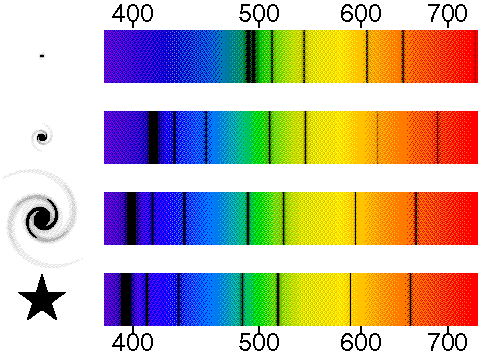
\includegraphics[width=0.6\textwidth]{redshift.png}\end{center}

En la figura pueden verse cuatro espectros de objetos astronómicos, los cuales
están ordenados desde el más lejano (arriba) al más cercano (abajo). La
estrella se encuentra en reposo respecto a la Tierra, y será nuestra referencia
para las líneas espectrales, que son, de izquierda a derecha (azul a rojo):
$393$, $397$, $410$, $434$, $486$, $518$, $589$ y $656$\,nm.

\begin{enumerate}
\item Utilizando las líneas espectrales mostradas, determine el corrimiento al
rojo para cada una de las líneas de los tres objetos distantes. 
\item Calcule el corrimiento al rojo de cada objeto como el promedio de los
corrimientos de cada línea de ese objeto.
\item Determine la velocidad de alejamiento de cada objeto, usando la expresión
aproximada 
\[z\simeq \frac vc.\]
Compare esos valores con los obtenidos a partir de la expresión exacta (debe
despejar $v$ de esta ecuación): 
\[z =  \sqrt{\frac{1+v/c}{1-v/c}} - 1\]
\item Usando la ley de Hubble calcule la distancia a la que se encuentran
esos tres objetos.
\end{enumerate}

\item {\bf{Densidad crítica (opcional)}}

Hemos visto que el Universo se encuentra en expansión, y lo hace con una
velocidad que depende de la distancia $d$, relación conocida como la ley de
Hubble:
\[v = H_0 d.\]
De esta manera, si tenemos una esfera de radio $R$ que se expande, la velocidad
a la cual la superficie de la esfera se aleja del centro de la misma es $v =
H_0 R$.
Con esto, y recordando la ecuación de la velocidad de escape
\[v_e = \sqrt{\frac{2 G M}{R}} \]
calcularemos la densidad crítica del Universo, es decir, la densidad para la
cual la fuerza de gravedad de la masa contenida sería capaz de detener la
expansión. Para ello,
\begin{enumerate}
\item obtenga la expresión para la masa $M$ de una esfera de radio $R$ y
volumen $V$ en función de la densidad $\rho$ (ayuda, recuerde $\rho=M/V$);
\item reemplace esta expresión para $M$ en la ecuación para la velocidad de
escape y despeje $\rho$;
\item si $\rho$ representa a la densidad crítica, la superficie de la esfera se
aleja del centro con la velocidad de escape. Puesto que a su vez se verifica la
ley de Hubble, tenemos que $v_e = H_0 R$. Reemplace este valor para la velocidad
de escape en la expresión para $\rho$ obtenida en el punto anterior;
\item verifique que el resultado obtenido, 
\[\rho_c = \frac{3 H_0^2}{8 \pi G}, \]
no depende del radio $R$;
\item finalmente, calcule el valor de $\rho_c$ en kg m$^{-3}$, tomando $H_0=71$
km s$^{-1}$ Mpc$^{-1}$. 
\item Exprese la densidad crítica en número de átomos de Hidrógeno por metro
cúbico, y en masas solares por parsec cúbico.
\item Si la densidad total del Universo fuera $\rho=2\,\rho_c$, ¿cuál sería el
posible destino del Universo? ¿Cuál sería la velocidad final de expansión en
este caso? 
\end{enumerate}

\end{enumerate}

\end{document}
%%%%
